\chapter{Le Modèle Standard}
\begin{fmffile}{chapitre1}

\section{Les particules élémentaires}

\begin{figure} \centering
  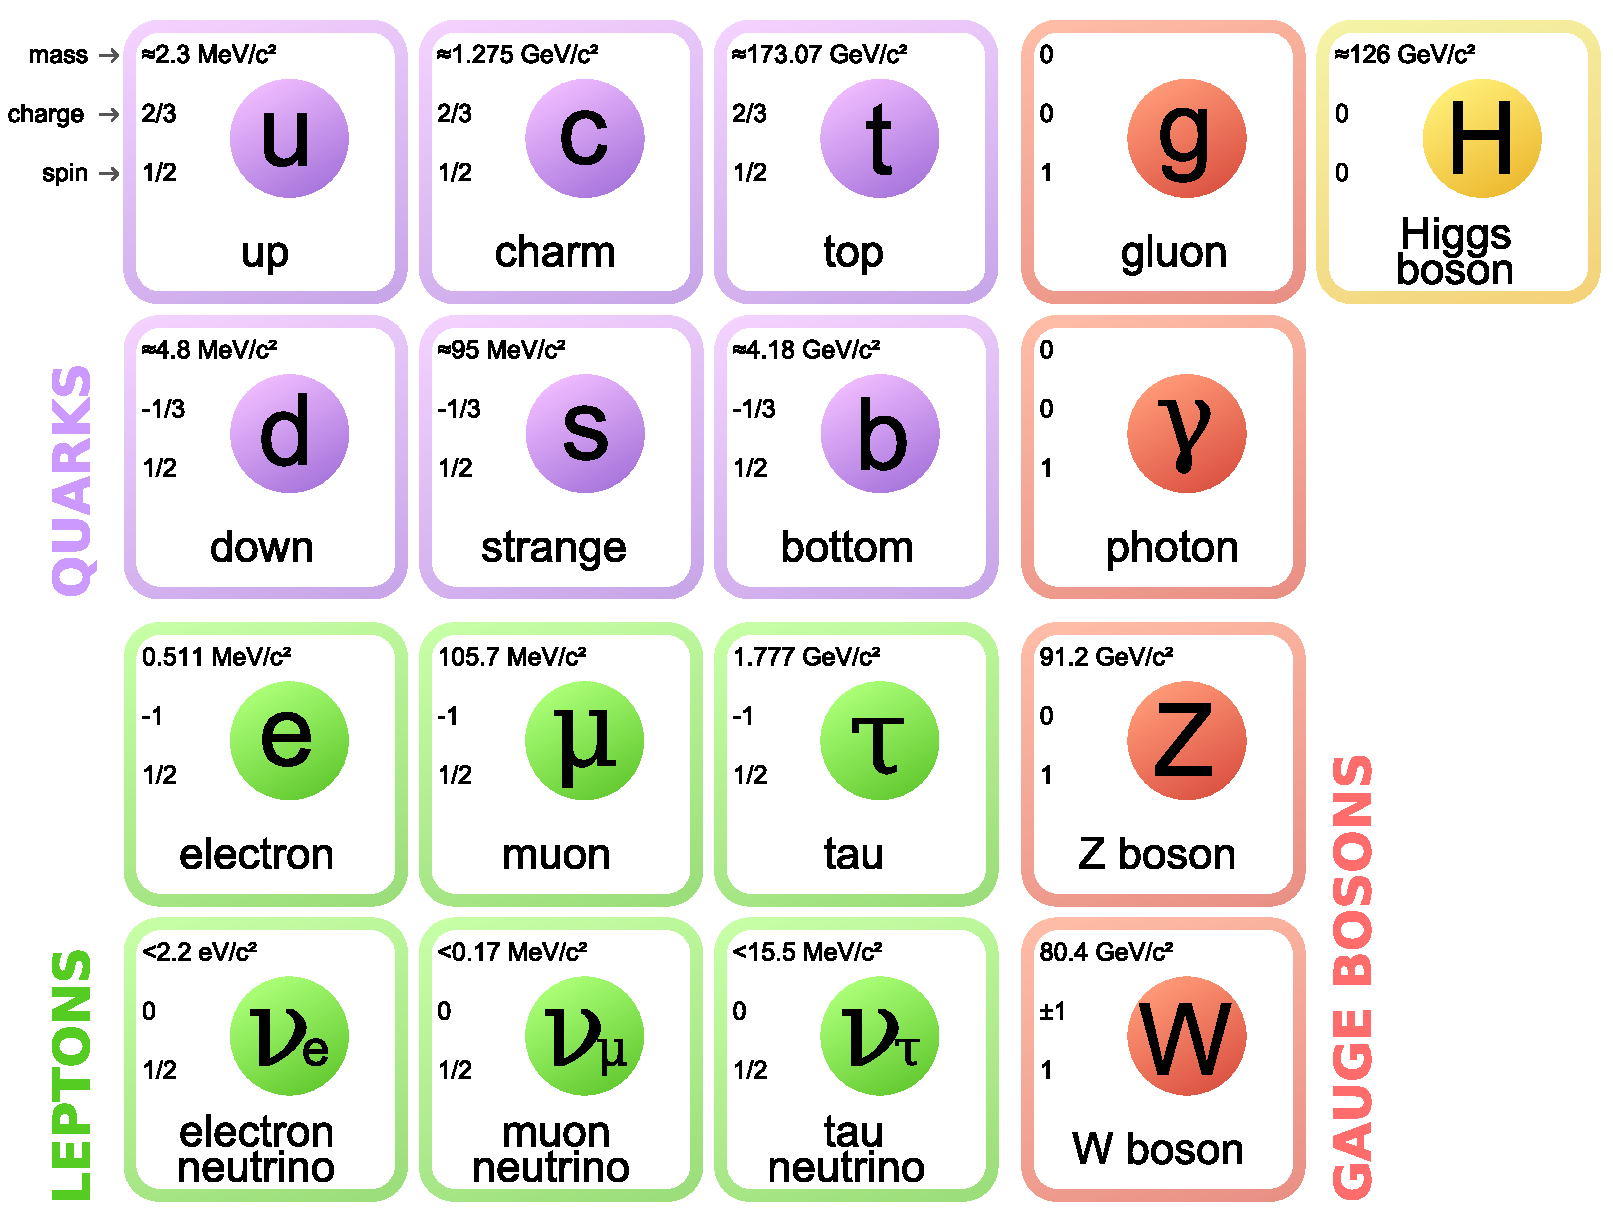
\includegraphics[height=0.33\textwidth]{Standard_Model_of_Elementary_Particles.pdf}
  \label{fig:sm}
  \caption{Les particules élémentaires du Modèle Standard.}
\end{figure}

\section{Paramétrisation théorique}

Avant de rentrer plus en détails dans la paramétrisation théorique du modèle standard, il convient dans un premier temps d'introduire le formalisme mathématique utilisé.

Comme on le verra par la suite, le modèle standard est bâti en exploitant les symétries qui existent entre les différentes particules élémentaires. Le formalisme le plus adapté a cette paramétrisation est le formalisme de Lagrange.

En mécanique classique, les équations d'Euler-Lagrange permettent d'obtenir les équations du mouvement d'une particule :
\begin{align}
  \frac{d}{dt} \left( \frac{\partial L}{\partial \dot{q_i}} \right) - \frac{\partial L}{\partial q_i} &= 0
\end{align}

où $q_i$ sont les coordonnées généralisées des particules, $t$ la variable temps, et $\dot{q_i} = dq_i / dt$. Le Lagrangien L est lui défini par une relation reliant l'énergie cinétique ($T$) et l'énergie potentielle ($V$) :
\begin{align*}
  L &= T - V
\end{align*}

Dans le cas de particules fondamentales, les coordonnées des particules ne sont plus discrète ($q_i(t)$), mais continue ($\phi(x, t)$). Le Lagrangien devient donc
\begin{align*}
  L(q_i, \dot{q_i}, t) \rightarrow \mathcal{L}\left(\phi, \frac{\partial \phi}{\partial x_\mu}, t\right)
\end{align*}

et les équations de Lagrange deviennent
\begin{align} \label{eq:lagrange}
  \frac{\partial}{\partial x_\mu}\left( \frac{\partial \mathcal{L}}{\partial \dot{\phi}} \right) - \frac{\partial \mathcal{L}}{\partial \phi} &= 0
\end{align}

C'est à l'aide de se formalisme que nous allons construire le modèle standard. En effet, une fois le Lagrangien établie, il est possible d'en dériver tout un jeu de règles, que l'on nomme règle de Feynmann, et qui permettent de quantifier l'interaction entre les particules élémentaire (vertex d'interaction) et leur propagation (propagateur). Plus de détails seront donnés par la suite, mais il est néanmoins déjà important de noter que, dans le Lagrangien :

\begin{enumerate}
  \item Les propagateurs sont associés aux termes quadratiques du Lagrangien
  \item Les autres termes correspondent aux vertex d'interactions. Les règles de Feynmann associées aux vertex sont simplement les termes dans $i\mathcal{L}$ qui contiennent les champs interagissant.
\end{enumerate}

\subsection{L'interaction électromagnétique (QED)} \label{sec:qed}

On considère le cas d'une particule de masse $m$ à laquelle on associe une fonction d'onde $\Psi(x)$. On défini le Lagrangien $L$ par
\begin{align} \label{eq:lagrangien_qed_simple}
  L &= i \bar{\Psi} \gmu \dmuc \Psi -m \bar{\Psi}\Psi
\end{align}

Ce choix, complètement arbitraire, permet de retrouver l'équation de Dirac\footnote{$\left(i \gmuc \dmu - m\right) \Psi = 0$} lorsque l'on applique \eqref{eq:lagrange}. Intéressons nous maintenant plus particulièrement aux symétries de ce Lagrangien. On s'aperçoit rapidement qu'il est invariant par changement de phase (aussi appelé jauge). En effet, en effectuant la transformation
\begin{align*}
  \Psi &\rightarrow \Psi^\prime = e^{i\theta}\Psi
\end{align*}
et en notant que
\begin{align*}
  \dmu \Psi &\rightarrow e^{i\theta}\dmu \Psi\\
  \bar{\Psi} = \Psi^\dagger \gzeroc &\rightarrow e^{-i\theta}\bar{\Psi}
\end{align*}
On a bien
\begin{align*}
  L &\rightarrow L^\prime = L
\end{align*}
On dit que le Lagrangien est invariant de jauge globale (la phase est la même dans tout l'espace temps). Les transformations du genre $U(\theta) = e^{i\theta}, \theta \in \mathbb{C}$ forment le groupe de symétrie unitaire Abélien $U(1)$.

Cette invariance a une conséquence très importante. En effet, d'après le théorème de N{\oe}ter, toute symétrie interne ou externe correspond à une quantité conservée. L'exemple le plus connu est probablement la conservation de l'énergie d'un système, cause directe de l'invariance temporelle. Dans le cas de notre Lagrangien, cette invariance conduit à l'équation de conservation
\begin{align} \label{eq:e_current}
  \dmu j^\mu &= 0 & \text{avec} && j^\mu &= -e \bar{\Psi} \gmuc \Psi
\end{align}
Le courant électronique $j^\mu$ est donc conservé, et on en déduit que la charge, défini par $Q = \int j^0 d^3x$ est aussi conservée.

Cette symétrie globale de jauge n'est pas la plus générale. Il serait en effet plus satisfaisant si la phase pouvait varier localement ($\theta \rightarrow \theta(x)$). Malheureusement, le Lagrangien \eqref{eq:lagrangien_qed_simple} n'est pas invariant lorsque l'on effectue la transformation
\begin{align*}
  \Psi \rightarrow e^{i\theta(x)}\Psi
\end{align*}
En effet, la dérivée de $\Psi$ se transforme maintenant comme
\begin{align} \label{eq:brisure_jauge_local}
  \dmu \Psi \rightarrow e^{i\theta(x)}\dmu\Psi + ie^{i\theta(x)}\Psi\dmu\theta(x)
\end{align}
Le terme $\dmu\theta(x)$ brise l'invariance de jauge. Il est cependant intéressant de voir ce qu'il se passe si on impose l'invariance du Lagrangien.

Pour se faire, il suffit de remplacer dérivée $\dmu$ dans la définition du Lagrangien par une autre dérivée $D_\mu$, appelée dérivée covariante. Cette nouvelle dérivée se transforme comme
\begin{align*}
  D_\mu\Psi &\rightarrow e^{i\theta(x)}D_\mu\Psi
\end{align*}
Afin de pouvoir écrire une telle dérivée, il est nécessaire d'introduire un nouveau champs vectoriel, $A_\mu$, qui se transforme de telle sorte d'annuler le terme en $\dmu \theta(x)$ dans \eqref{eq:brisure_jauge_local}. On défini la dérivée covariante par\footnote{le terme $e$ (charge électrique) est purement conventionnel}
\begin{align*}
  D_\mu &= \dmu - ieA_\mu
\end{align*}
où $A_\mu$ se transforme comme
\begin{align} \label{eq:photon_jauge_transformation}
  A_\mu &\rightarrow A_\mu + \frac{1}{e}\dmu\theta(x)
\end{align}
En remplaçant $\dmu$ par $D_\mu$, on obtient le Lagrangien invariant de jauge local
\begin{align*}
  L &= \Psib\left(i\gmuc\dmu - m\right)\Psi + e\Psib \gmuc \Psi A_\mu
\end{align*}

En forçant le Lagrangien à être invariant de jauge local, nous sommes obligé d'introduire un nouveau champs vectoriel (champs de jauge): c'est le photon. Afin de vraiment interpréter ce nouveau champs comme le photon, il est nécessaire d'ajouter dans le Lagrangien un terme correspondant à l'énergie cinétique du photon. Le seul candidat invariant lors de la transformation \eqref{eq:photon_jauge_transformation} doit être construit à partir du tenseur
\begin{align*}
  F_{\mu\nu} &= \dmu A_\nu - \partial_\nu A_\mu
\end{align*}

On obtient donc finalement le Lagrangien décrivant l'interaction électromagnétique
\begin{align} \label{eq:l_qed}
  L_{\text{QED}} &= \Psib\left(i\gmuc\dmu - m\right)\Psi + e\Psib \gmuc \Psi A_\mu - \frac{1}{4} F_{\mu\nu}F^{\mu\nu}
\end{align}
Un dernier point reste à remarquer. Il n'est pas possible d'ajouter un terme $\frac{1}{2}m^2A_\mu A^\mu$ sans violer l'invariance locale de jauge. Le photon doit donc être sans masse.

\bigskip

Imposer l'invariance locale de jauge du Lagrangien nous a forcé à introduire une nouvelle particule, sans masse : le photon. Nous verrons par la suite qu'imposer l'invariance locale de jauge nous permet de décrire aussi bien l'interaction faible (via l'unification électrofaible) que l'interaction forte.

\subsection{L'interaction forte (QCD)} \label{sec:qcd}

Le modèle des quarks est une grande réussite, et a permis d'expliquer de façon élégante la prolifération de nouvelles particules ($\pi^{0/+/-}$, $K$, $\eta$, \ldots). Cependant, la découverte du $\Delta^{++}$ en 1951 remet en cause le modèle. En effet, cet hadron est composé de trois quarks $u$. Le principe d'exclusion de Pauli interdit deux particules de spin $\frac{1}{2}$ d'être dans le même état quantique. Étant de spin $\frac{3}{2}$, $\Delta^{++}$ est forcément composée de deux $u$ de même spin, ce qui n'est pas autorisé par le principe d'exclusion.

La solution à ce problème est d'introduire un nouveau nombre quantique, similaire à la charge électrique : la charge de couleur. Un quark peut donc exister en trois couleurs différentes : rouge ($R$), vert ($V$), bleu ($B$), et un anti-quark en cyan ($\bar{R}$), magenta ($\bar{V}$) et jaune ($\bar{B}$)\footnote{Par analogie à la synthèse des couleurs}. En réalité, $\Delta^{++}$ est composé de $u_R u_V u_B$, ce qui permet de s'affranchir du principe d'exclusion de Pauli : chaque quark est dans un état quantique différent. Ce nouveau nombre quantique permet aussi d'expliquer pourquoi il n'existe pas d'état lié $qq$ ou $\bar{q}\bar{q}$ : un état lié de quarks doit apparaître "blanc", c'est-à-dire non coloré. Ainsi, un méson est toujours un état lié $q_i\bar{q}_i$, où $i$ est la couleur ($R$, $V$ ou $B$), et un hadron un état $q_R q_V q_B$ ou $\bar{q}_{\bar{R}} \bar{q}_{\bar{V}} \bar{q}_{\bar{B}}$.

\bigskip

Le Lagrangien de la QCD est basée sur la même idée que section \ref{sec:qed}, à la seule différence que l'on remplace la symétrie de jauge $U(1)$ par $SU(3)$, puisque chaque quark existe en trois couleurs différentes. Le Lagrangien devient donc
\begin{align*}
  L &= \bar{q}_i^j\left(i\dmu\gmuc -m\right)q_i^j
\end{align*}
où $i$ représente la charge de couleur et $j$ la saveur du quark.

Comme précédemment, on requiert que le Lagrangien soit invariant locale de jauge, c'est-à-dire qu'il soit invariant lorsque l'on applique la transformation
\begin{align} \label{eq:su3_jauge}
  q(x) \rightarrow Uq(x) = e^{i \theta_a(x) T_a}q(x) \simeq \left(1 + i\theta_a(x) T_a\right)q(x)
\end{align}
où $T_a$ sont un ensemble de 8 matrices, et $\theta_a$ sont les paramètres du groupe. Un choix conventionnel pour $T_a$ est $\frac{\lambda_a}{2}$, où $\lambda$ sont les matrices de Gell-Mann. Ce groupe est non Abélien puisque les générateurs du groupe $T_a$ ne commutent pas entre eux :
\begin{align*}
  \left[T_i, T_j\right] &= i f_{ijk} T_k
\end{align*}
Les coefficients $f_{ijk}$ sont réels et sont appelées constantes de structure du groupe. Après la transformation \eqref{eq:su3_jauge}, on a
\begin{align*}
  \dmu q \rightarrow (1 + i\theta_a(x) T_a)q + iT_aq\dmu\theta_a(x)
\end{align*}
L'invariance de jauge est donc ici aussi violée par le terme en $\dmu\theta_a$. On procède de la même façon que pour la QED. On introduit la dérivée covariante
\begin{align*}
  D_\mu &= \dmu + igT_aG_\mu^a
\end{align*}
Cette fois, nous sommes obligés d'introduire non pas un champs vectoriel, mais huit. Ces nouveaux champs se transforment de la façon suivante :
\begin{align*}
  G_\mu^a \rightarrow G_\mu^a - \frac{1}{g} \dmu \theta_a - f_{abc}\theta_bG_\mu^c
\end{align*}
Le dernier terme est nécessaire puisque $SU(3)$ est un groupe non Abélien. Pour finir, il suffit d'ajouter les termes d'énergie cinétique pour chacun des huit nouveaux champs au Lagrangien pour obtenir la paramétrisation de la QCD :
\begin{align} \label{eq:l_qcd}
  L_{\text{QCD}} &= \bar{q}_i^j\left(i\dmu\gmuc -m\right)q_i^j - g\left(\bar{q}_i^j\gmuc T_a q_i^j\right)G_\mu^a - \frac{1}{4}G_{\mu\nu}^aG_a^{\mu\nu}
\end{align}

Le tenseur $G_{\mu\nu}$ est défini de façon analogue à $F_{\mu\nu}$, mais, étant donné le caractère non Abélien du groupe, des termes supplémentaires sont présent :
\begin{align*}
  G_{\mu\nu}^a &= \dmu G_\nu^a - \partial_\nu G_\mu^a - g f_{abc} G_\mu^b G_\nu^c
\end{align*}

On peut finalement interpréter les huit nouveaux champs vectoriels comme les huit gluons du Modèle Standard. Comme pour le photon, il n'est pas possible d'introduire un terme de masse dans \eqref{eq:l_qcd} sans briser l'invariance locale de jauge. Les gluons doivent donc être sans masse.

Une des propriétés remarquables du tenseur $G_{\mu\nu}^a$ est que, contrairement à $F_{\mu\nu}$, il contient des termes d'auto-interaction ($\propto G_\mu^b G_\nu^c$). En effet, les gluons étant médiateur de l'interaction force et portant eux même une charge de couleur, ils peuvent interagir entre eux, comme on peut le voir figure \ref{fig:gluon_self_interaction}.

\begin{figure} \centering
  \subcaptionbox{\label{fig:3_gluons_vertex}}[.4\linewidth]{
  \begin{fmfgraph*}(200,100)
    \fmfpen{0.5}
    \fmfleft{i1}
    \fmfright{o1,o2}
    \fmf{gluon}{i1,v1,o1}
    \fmf{gluon}{v1,o2}
    \fmfdot{v1}
  \end{fmfgraph*}}\qquad%
  \subcaptionbox{\label{fig:4_gluons_vertex}}[.4\linewidth]{
  \begin{fmfgraph*}(200,100)
    \fmfpen{0.5}
    \fmfleft{i1,i2}
    \fmfright{o1,o2}
    \fmf{gluon}{i1,v1,o1}
    \fmf{gluon}{i2,v1,o2}
    \fmfdot{v1}
  \end{fmfgraph*}}
  \caption{Vertex d'interaction à 3 (\protect\subref{fig:3_gluons_vertex}) et 4 (\protect\subref{fig:4_gluons_vertex}) gluons.}
  \label{fig:gluon_self_interaction}
\end{figure}

\subsection{L'unification électrofaible}

On a pu voir précédemment que les médiateurs de l'interaction faible sont les bosons chargés $W^{+/-}$, ainsi que le boson neutre $Z^0$. On peut voir figure \ref{fig:w_decay} la désintégration d'un boson $W$ en $e\nu$.

\begin{figure}[b] \centering
  \subcaptionbox{$W^- \rightarrow e^- \bar{\nu}_e$}[.4\linewidth]{
  \begin{fmfgraph*}(200,100)
    \fmfpen{0.5}
    \fmfleft{i1}
    \fmfright{o1,o2}
    \fmf{boson,label=$W^-$}{i1,v1}
    \fmf{fermion}{o1,v1,o2}
    \fmfdot{v1}
    \fmflabel{$e^-$}{o2}
    \fmflabel{$\bar{\nu}_e$}{o1}
  \end{fmfgraph*}}\qquad%
  \subcaptionbox{$W^+ \rightarrow e^+ \nu_e$}[.4\linewidth]{
  \begin{fmfgraph*}(200,100)
    \fmfpen{0.5}
    \fmfleft{i1}
    \fmfright{o1,o2}
    \fmf{boson,label=$W^+$}{i1,v1}
    \fmf{fermion}{o1,v1,o2}
    \fmfdot{v1}
    \fmflabel{$e^+$}{o1}
    \fmflabel{$\nu_e$}{o2}
  \end{fmfgraph*}}
  \caption{Désintégration des bosons $W^{+/-}$ en $e\nu$}
  \label{fig:w_decay}
\end{figure}

De façon analogique au courant électromagnétique \eqref{eq:e_current}, on introduit le courant faible chargé

\begin{align*}
  j^\mu_{\text{w}} &= G \bar{u}_\nu \gmuc u_e
\end{align*}

Ce courant est invariant lors des transformations de parité. Malheureusement, bien que permettant d'expliquer la plupart des observations sur la désintégration $\beta$, cette formulation du courant échoue sur d'autre point. En effet, en étudiant la désintégration $\beta$ de nombreux atomes (tel que le cobalt), il s'est avéré que l'interaction faible ne fait apparaître que des neutrino d'hélicité gauche ($\nu_L$) ou des anti-neutrino d'hélicité droite ($\bar{\nu}_R$) : ceci est une violation directe de l'invariance de la parité, et il est nécessaire que le courant faible reflète ceci.

Parmi les invariants de Lorentz qui ne sont pas invariants par parité, on trouve les structures $\frac{1}{2}\gmuc(1 - \gfivec)$ et $\frac{1}{2}\gmuc(1 + \gfivec)$. Ces deux structures sont respectivement les projecteurs de chiralité gauche et droite. Lorsque la masse devient négligeable devant l'énergie, la chiralité se confond avec l'hélicité. Le neutrino n'ayant pas de masse, le projecteur de chiralité projette aussi l'hélicité. L'expérience nous oblige donc à choisir la structure $\frac{1}{2}\gmuc(1 - \gfivec)$ (structure $V - A$, pour Vecteur - Axial), puisque l'interaction faible ne couple uniquement que les neutrino d'hélicité gauche. Le courant faible chargé devient alors

\begin{align}
  j^\mu_{\text{w}} &= G \bar{u}_\nu \frac{1}{2} \gmuc \left(1 - \gfivec \right) u_e
\end{align}

On peut ré-exprimer le courant faible en décomposant $u$ en $u_L$ et $u_R$. On obtient alors
\begin{align*}
&\left. \begin{aligned} 
  J_\mu &= J_\mu^+ = \bar{u}_\nu \frac{1}{2} \gmu \left(1 - \gfivec \right) u_e \\
   &\equiv \bar{\nu} \frac{1}{2} \gmu \left(1 - \gfivec \right) e = \bar{\nu}_L \gmu e_L
\end{aligned} \right\}\,W^+ \rightarrow e^+ \nu_e\\
&\left. \begin{aligned}
  J_\mu^\dagger &= J_\mu^- = \bar{u}_e \frac{1}{2} \gmu \left(1 - \gfivec \right) u_\nu \\
   &\equiv \bar{e} \frac{1}{2} \gmu \left(1 - \gfivec \right) \nu = \bar{e}_L \gmu \nu_L
\end{aligned} \right\}\,W^- \rightarrow e^- \bar{\nu}_e
\end{align*}

On peut réécrire de façon plus succincte l'équation précédente en introduisant un nouveau doublet, $\chi_L$, défini comme
\begin{align*}
  \chi_L = \colvec{2}{\nu}{e^-}_L
\end{align*}
ainsi que les opérateur $\tau_+$ et $\tau_-$, défini comme $\tau_{\pm} = \frac{1}{2}\left( \tau_1 \pm i\tau_2 \right)$ ($\tau_i$ sont les trois matrices de Pauli). Les courants faibles chargés peuvent être réécrit comme
\begin{align*}
  J_\mu^+ &= \bar{\chi}_L \gmu \tau_+ \chi_L \\
  J_\mu^- &= \bar{\chi}_L \gmu \tau_- \chi_L
\end{align*}
La structure $V-A$ de l'interaction faible disparaît pour laisser apparaître une interaction purement vectorielle entre fermions d'hélicité gauche, interaction ressemblant fortement à celle de QED. Cette observation nous laisse entrevoir une possible unification entre l'interaction faible et électromagnétique : l'interaction électrofaible.

\bigskip

On a défini $J_\mu^{\pm}$ à l'aide des matrices de Pauli, générateurs du groupe de symétrie $SU(2)$. Essayons de définir le courant neutre $J_\mu^3$ :
\begin{align*}
  J_\mu^3 &= \bar{\chi}_L \gmu \frac{1}{2} \tau_3 \chi_L = \rowvec{2}{\bar{\nu}}{e^+}_L \gmu \frac{1}{2} \begin{pmatrix}
    1 & 0 \\
    0 & -1
  \end{pmatrix} \colvec{2}{\nu}{e^-}_L \\
  &= \frac{1}{2} \bar{\nu}_L \gmu \nu_L - \frac{1}{2} e^+_L \gmu e^-_L
\end{align*}

Continuons cependant dans cette voie. On forme avec $J_\mu^i$, $i = 1 \ldots 3$ un triplet "d'isopin" de courant faible
\begin{align*}
  J_\mu^i &= \bar{\chi}_L \gmu \frac{1}{2} \tau_i \chi_L
\end{align*}

On défini l'équivalent de la charge par $T^i = \int J_0^I d^3x$. Ces charges forment les générateurs du groupe $SU(2)_L$, avec comme relation de commutation
\begin{align*}
  \left[ T^i, T^j \right] &= i \epsilon_{ijk}T^k
\end{align*}

On peut être tenter d'interpréter $J_\mu^3$ comme le courant faible neutre associé au $Z^0$. Malheureusement, ceci est incorrect, puisque le courant que l'on vient d'écrire ne couple que des particules d'hélicité gauche, contrairement au $Z^0$, qui couple indifféremment les hélicités gauche et droite. Cependant, le courant électromagnétique est aussi un courant neutre, qui couple les deux hélicités. On rappelle que $ej^{EM}_\mu = e\Psib \gmu Q \Psi$, où $Q$ est l'opérateur de charge.

Afin de sauver la symétrie $SU(2)_L$, nous sommes contraint de faire intervenir l'interaction électromagnétique afin d'avoir un courant neutre faible convenable. Pour ce faire, nous étendons la symétrie en formant deux combinaisons orthogonales qui ont des transformations défini sous $SU(2)_L$ : la première combinaison, $J_\mu^3$ permet de former le triplet d'isopin. La seconde combinaison $j_\mu^Y$ doit rester invariant sous $SU(2)_L$ : c'est courant neutre d'hypercharge (on généralise ici la charge électrique), donné par
\begin{align*}
  j_\mu^Y &= \Psib \gmu Y \Psi
\end{align*}
et on défini l'hypercharge $Y$ par une relation reliant la charge électrique $Q$ et la "charge" neutre faible $T^3$ :
\begin{align*}
  Q &= T^3 + \frac{Y}{2}
\end{align*}
$Y$ est ainsi un générateur du groupe $U(1)_Y$. On étend ainsi le groupe $SU(2)_L$ au groupe de symétrie $SU(2)_L \times U(1)_Y$. On a alors les doublets d'isopin $\chi_L$, composés des fermions de même famille d'hélicité gauche et qui se transforment sous $SU(2)_L$ et $U(1)_Y$. Enfin, on classifie les fermions d'hélicité droit dans des singlets d'isospin, invariant sous $SU(2)_L$ et qui se transforment sous $U(1)_Y$.
\begin{align*}
  \chi_L &= \colvec{2}{\nu}{e}_L, \colvec{2}{u}{d}_L & & \text{doublet d'isospin} \\
  \Psi_R &= e_R, u_R \text{ ou } d_R & & \text{singlet d'isospin}
\end{align*}

\bigskip

On procède maintenant de la même façon que pour QED et QCD. On introduit le Lagrangien $L$ défini par
\begin{align*}
  L &= \bar{\chi}_L\left(i\gmuc\dmu - m\right)\chi_L + \Psib_R \left(i\gmuc\dmu - m\right) \Psi_R
\end{align*}
$\chi_L$ et $\Psi_R$ se transforment respectivement sous $SU(2)_L \times U(1)_Y$ et $U(1)_Y$, selon les relations
\begin{align*}
  \chi_L &\rightarrow \chi^\prime_L = e^{i\vec{\theta}(x) \cdot \vec{T}\,+\,i\iota(x) Y}\chi_L \\
  \Psi_R &\rightarrow \Psi_R^\prime = e^{i\iota(x) Y}\Psi_R
\end{align*}

On impose maintenant l'invariance locale de jauge au Lagrangien. Pour ce faire, la première étape est de remplacer la dérivée par deux dérivées covariantes $D_\mu^i$, définies par
\begin{align*}
  D_\mu^1 &= \dmu + ig_1\frac{1}{2}\vec{\tau} \cdot \vec{W}_\mu + ig_2 \frac{Y}{2} B_\mu\\
  D_\mu^2 &= \dmu + ig_2 \frac{Y}{2} B_\mu
\end{align*}

Encore une fois, imposer l'invariance locale de jauge nous force à introduire quatre nouveaux champs vectoriels, un triplet d'isospin $\vec{W}_\mu$ et un singlet $B_\mu$. Ces nouveaux champs se transforment comme
\begin{align*}
  B_\mu &\rightarrow B_\mu - \frac{1}{g_2} \dmu \iota(x) \\
  \vec{W}_\mu &\rightarrow \vec{W}_\mu - \frac{1}{g_1} \dmu \vec{\theta}(x) - \vec{\theta}(x) \times \vec{W}_\mu
\end{align*}
Afin de compléter le Lagrangien, il nous reste à ajouter les termes cinétiques des quatre nouveaux champs. On introduit donc quatre tenseurs, défini par
\begin{align*}
  B_{\mu\nu} &= \dmu B_\nu - \partial_\nu B_\mu\\
  \vec{W}_{\mu\nu} &= \dmu\vec{W}_\nu - \partial_\nu \vec{W}_\mu - g_1 \vec{W}_\mu \times \vec{W}_\nu
\end{align*}

En ajoutant tous les termes ensemble, on obtient le Lagrangien de l'interaction électrofaible :
\begin{align*}
 L_{\text{EWK}} = &\bar{\chi}_L \gmuc \left( i\dmu - g_1 \frac{1}{2} \vec{\tau} \cdot \vec{W}_\mu - g_2 \frac{Y}{2} B_\mu \right) \chi_L + \Psib_R \gmuc \left( i\dmu - g_2 \frac{Y}{2} B_\mu \right) \Psi_R \\
 &- \frac{1}{4}B_{\mu\nu}B^{\mu\nu} - \frac{1}{4}\vec{W}_{\mu\nu} \cdot \vec{W}^{\mu\nu}
\end{align*}

Les termes en $m\bar{\chi}_L\chi_L$ et $m\Psib\Psi$ ont disparu du Lagrangien final. En effet, ces termes ne sont pas invariant sous transformation locale de jauge : les fermions perdent donc leur masse lors de l'unification électrofaible. De même, comme pour le photon ou les gluons, il n'est pas possible d'ajouter des termes de masse pour les nouveaux bosons introduit : ils doivent donc être sans masse.

\bigskip

Cette formulation de l'interaction faible permet de retrouver les deux bosons chargés de l'interaction faible, $W^{+/-}$, défini par
\begin{align*}
  W^{\pm} &= \frac{1}{\sqrt{2}} \left(W^1 \mp iW^2 \right)
\end{align*}
Il n'est cependant pas possible d'interpréter $W^3$ comme le boson $Z^0$, ni $B$ comme le photon, pour les mêmes raisons que précédemment. Tout n'est pas perdu, et nous verrons par la suite que ces deux champs vectoriels se mélangent pour former le $Z^0$ et le photon.

\bigskip

Comme formulée actuellement, la théorie électrofaible a deux problèmes
\begin{enumerate}
  \item L'interaction électrofaible ne couple que les fermions d'une même famille. Si cela ne pose aucun soucis théorique, l'expérience montre que l'interaction faible couple des familles différentes\footnote{Par exemple, on observe $K^+ \rightarrow \pi^+ \pi^0$ où un quark $s$ se transforme en quark $d$}. Cabibbo apportât la solution en 1963 : il postula que les états propre de masse des quarks n'étaient pas états propres de l'interaction faible. Autrement dit, les quarks que nous observons sont en réalité un mélange entre les quarks états propre de l'interaction faible. Si on désigne avec un $^\prime$ les états propres de l'interaction faible, l'idée de Cabibbo s'écrit
  \begin{align*}
    \colvec{2}{d^\prime}{s^\prime} &= \begin{pmatrix}
      \cos{\theta_c} & \sin{\theta_c} \\
      - \sin{\theta_c} & \cos{\theta_c}
    \end{pmatrix} \colvec{2}{d}{s}
  \end{align*}
  où $\theta_c$ est l'angle de Cabibbo, et représente le mélange entre les différentes saveur de quarks. En réalité, le passage de l'espace vectoriel formé par les états propres de l'interaction faible à l'espace vectoriel formé par les états propres de masse s'effectue par une rotation d'angle $\theta_c$. La valeur de $\theta_c$ est déterminée de façon très précise par l'expérience à \SI{13.015}{\degree}.
  
  Cette matrice a ensuite été étendue aux trois générations de quarks du Modèle Standard par Kobayashi et Maskawa pour devenir une matrice $3 \times 3$ : la matrice CKM.
  \begin{align*}
    \colvec{3}{d^\prime}{s^\prime}{b^\prime} &= \begin{pmatrix} V_{ud} & V_{us} & V_{ub} \\ V_{cd} & V_{cs} & V_{cb} \\ V_{td} & V_{ts} & V_{tb} \end{pmatrix} \colvec{3}{d}{s}{b}
  \end{align*}
  
  
  \item Higgs
\end{enumerate}

\end{fmffile}
